% Options for packages loaded elsewhere
\PassOptionsToPackage{unicode}{hyperref}
\PassOptionsToPackage{hyphens}{url}
\PassOptionsToPackage{dvipsnames,svgnames*,x11names*}{xcolor}
%
\documentclass[
]{article}
\usepackage{lmodern}
\usepackage{amssymb,amsmath}
\usepackage{ifxetex,ifluatex}
\ifnum 0\ifxetex 1\fi\ifluatex 1\fi=0 % if pdftex
  \usepackage[T1]{fontenc}
  \usepackage[utf8]{inputenc}
  \usepackage{textcomp} % provide euro and other symbols
\else % if luatex or xetex
  \usepackage{unicode-math}
  \defaultfontfeatures{Scale=MatchLowercase}
  \defaultfontfeatures[\rmfamily]{Ligatures=TeX,Scale=1}
\fi
% Use upquote if available, for straight quotes in verbatim environments
\IfFileExists{upquote.sty}{\usepackage{upquote}}{}
\IfFileExists{microtype.sty}{% use microtype if available
  \usepackage[]{microtype}
  \UseMicrotypeSet[protrusion]{basicmath} % disable protrusion for tt fonts
}{}
\makeatletter
\@ifundefined{KOMAClassName}{% if non-KOMA class
  \IfFileExists{parskip.sty}{%
    \usepackage{parskip}
  }{% else
    \setlength{\parindent}{0pt}
    \setlength{\parskip}{6pt plus 2pt minus 1pt}}
}{% if KOMA class
  \KOMAoptions{parskip=half}}
\makeatother
\usepackage{xcolor}
\IfFileExists{xurl.sty}{\usepackage{xurl}}{} % add URL line breaks if available
\IfFileExists{bookmark.sty}{\usepackage{bookmark}}{\usepackage{hyperref}}
\hypersetup{
  pdftitle={Soluciones PRELIMINARES: Entrega 4 y FINAL. Problemas y Talleres MATIII Estadística grado informática 2019-2020},
  pdfauthor={Ricardo Alberich},
  colorlinks=true,
  linkcolor=red,
  filecolor=Maroon,
  citecolor=blue,
  urlcolor=blue,
  pdfcreator={LaTeX via pandoc}}
\urlstyle{same} % disable monospaced font for URLs
\usepackage[margin=1in]{geometry}
\usepackage{color}
\usepackage{fancyvrb}
\newcommand{\VerbBar}{|}
\newcommand{\VERB}{\Verb[commandchars=\\\{\}]}
\DefineVerbatimEnvironment{Highlighting}{Verbatim}{commandchars=\\\{\}}
% Add ',fontsize=\small' for more characters per line
\usepackage{framed}
\definecolor{shadecolor}{RGB}{248,248,248}
\newenvironment{Shaded}{\begin{snugshade}}{\end{snugshade}}
\newcommand{\AlertTok}[1]{\textcolor[rgb]{0.94,0.16,0.16}{#1}}
\newcommand{\AnnotationTok}[1]{\textcolor[rgb]{0.56,0.35,0.01}{\textbf{\textit{#1}}}}
\newcommand{\AttributeTok}[1]{\textcolor[rgb]{0.77,0.63,0.00}{#1}}
\newcommand{\BaseNTok}[1]{\textcolor[rgb]{0.00,0.00,0.81}{#1}}
\newcommand{\BuiltInTok}[1]{#1}
\newcommand{\CharTok}[1]{\textcolor[rgb]{0.31,0.60,0.02}{#1}}
\newcommand{\CommentTok}[1]{\textcolor[rgb]{0.56,0.35,0.01}{\textit{#1}}}
\newcommand{\CommentVarTok}[1]{\textcolor[rgb]{0.56,0.35,0.01}{\textbf{\textit{#1}}}}
\newcommand{\ConstantTok}[1]{\textcolor[rgb]{0.00,0.00,0.00}{#1}}
\newcommand{\ControlFlowTok}[1]{\textcolor[rgb]{0.13,0.29,0.53}{\textbf{#1}}}
\newcommand{\DataTypeTok}[1]{\textcolor[rgb]{0.13,0.29,0.53}{#1}}
\newcommand{\DecValTok}[1]{\textcolor[rgb]{0.00,0.00,0.81}{#1}}
\newcommand{\DocumentationTok}[1]{\textcolor[rgb]{0.56,0.35,0.01}{\textbf{\textit{#1}}}}
\newcommand{\ErrorTok}[1]{\textcolor[rgb]{0.64,0.00,0.00}{\textbf{#1}}}
\newcommand{\ExtensionTok}[1]{#1}
\newcommand{\FloatTok}[1]{\textcolor[rgb]{0.00,0.00,0.81}{#1}}
\newcommand{\FunctionTok}[1]{\textcolor[rgb]{0.00,0.00,0.00}{#1}}
\newcommand{\ImportTok}[1]{#1}
\newcommand{\InformationTok}[1]{\textcolor[rgb]{0.56,0.35,0.01}{\textbf{\textit{#1}}}}
\newcommand{\KeywordTok}[1]{\textcolor[rgb]{0.13,0.29,0.53}{\textbf{#1}}}
\newcommand{\NormalTok}[1]{#1}
\newcommand{\OperatorTok}[1]{\textcolor[rgb]{0.81,0.36,0.00}{\textbf{#1}}}
\newcommand{\OtherTok}[1]{\textcolor[rgb]{0.56,0.35,0.01}{#1}}
\newcommand{\PreprocessorTok}[1]{\textcolor[rgb]{0.56,0.35,0.01}{\textit{#1}}}
\newcommand{\RegionMarkerTok}[1]{#1}
\newcommand{\SpecialCharTok}[1]{\textcolor[rgb]{0.00,0.00,0.00}{#1}}
\newcommand{\SpecialStringTok}[1]{\textcolor[rgb]{0.31,0.60,0.02}{#1}}
\newcommand{\StringTok}[1]{\textcolor[rgb]{0.31,0.60,0.02}{#1}}
\newcommand{\VariableTok}[1]{\textcolor[rgb]{0.00,0.00,0.00}{#1}}
\newcommand{\VerbatimStringTok}[1]{\textcolor[rgb]{0.31,0.60,0.02}{#1}}
\newcommand{\WarningTok}[1]{\textcolor[rgb]{0.56,0.35,0.01}{\textbf{\textit{#1}}}}
\usepackage{graphicx,grffile}
\makeatletter
\def\maxwidth{\ifdim\Gin@nat@width>\linewidth\linewidth\else\Gin@nat@width\fi}
\def\maxheight{\ifdim\Gin@nat@height>\textheight\textheight\else\Gin@nat@height\fi}
\makeatother
% Scale images if necessary, so that they will not overflow the page
% margins by default, and it is still possible to overwrite the defaults
% using explicit options in \includegraphics[width, height, ...]{}
\setkeys{Gin}{width=\maxwidth,height=\maxheight,keepaspectratio}
% Set default figure placement to htbp
\makeatletter
\def\fps@figure{htbp}
\makeatother
\setlength{\emergencystretch}{3em} % prevent overfull lines
\providecommand{\tightlist}{%
  \setlength{\itemsep}{0pt}\setlength{\parskip}{0pt}}
\setcounter{secnumdepth}{5}
\renewcommand{\contentsname}{Contenidos}

\title{Soluciones PRELIMINARES: Entrega 4 y FINAL. Problemas y Talleres MATIII
Estadística grado informática 2019-2020}
\author{Ricardo Alberich}
\date{13-05-2020}

\begin{document}
\maketitle

{
\hypersetup{linkcolor=blue}
\setcounter{tocdepth}{4}
\tableofcontents
}
\hypertarget{entrega-4-problemas-estaduxedstica-inferencial-2}{%
\section{Entrega 4 Problemas: Estadística Inferencial
2}\label{entrega-4-problemas-estaduxedstica-inferencial-2}}

Contestad en GRUPOS del proyecto a los siguientes problemas y cuestiones
en un fichero Rmd y su salida en html o pdf.

Cambien podéis incluir capturas de problemas hechos en papel. Cada
pregunta vale lo mismo y se reparte la nota entre sus apartados.

\hypertarget{problema-1-contraste-de-proporciones-de-dos-muestras-independientes.}{%
\subsection{Problema 1: Contraste de proporciones de dos muestras
independientes.}\label{problema-1-contraste-de-proporciones-de-dos-muestras-independientes.}}

Queremos comparar las proporciones de aciertos de dos redes neuronales
que detectan tipos si una foto con un móvil de una avispa es una
\href{https://es.wikipedia.org/wiki/Vespa_velutina}{avispa velutina o
asiática}. Esta avispa en una especie invasora y peligrosa por el veneno
de su picadura. Para ello disponemos de una muestra de 1000 imágenes de
insectos etiquetadas como avispa velutina y no velutina.

\href{http://bioinfo.uib.es/~recerca/MATIIIGINF/velutina}{Aquí tenéis el
acceso a los datos}. Cada uno está en fichero los aciertos están
codificados con 1 y los fallos con 0.

Se pide:

\begin{enumerate}
\def\labelenumi{\arabic{enumi}.}
\tightlist
\item
  Cargad los datos desde el servidos y calcular el tamaño de las
  muestras y la proporción de aciertos de cada muestra.
\item
  Contrastad si hay evidencia de que las las proporciones de aciertos
  del algoritmo 1 son mayores que las del algoritmo 2. Definid bien las
  hipótesis y las condiciones del contraste. Tenéis que hacer el
  contraste con funciones de \texttt{R} y resolver el contrate con el
  \(p\)-valor.
\item
  Calculad e interpretar los intervalos de confianza para la diferencia
  de proporciones asociados al test anterior, con funciones de R.
\end{enumerate}

\hypertarget{soluciuxf3n}{%
\subsubsection{Solución}\label{soluciuxf3n}}

\begin{Shaded}
\begin{Highlighting}[]
\NormalTok{algoritmo1=}\KeywordTok{read.table}\NormalTok{(}\StringTok{"http://bioinfo.uib.es/~recerca/MATIIIGINF/velutina/algoritmo1.csv"}\NormalTok{)}
\NormalTok{algoritmo2=}\KeywordTok{read.table}\NormalTok{(}\StringTok{"http://bioinfo.uib.es/~recerca/MATIIIGINF/velutina/algoritmo2.csv"}\NormalTok{)}
\end{Highlighting}
\end{Shaded}

Proporción aciertos de cada algoritmo

\begin{Shaded}
\begin{Highlighting}[]
\NormalTok{n1=}\KeywordTok{dim}\NormalTok{(algoritmo1)[}\DecValTok{1}\NormalTok{]}
\NormalTok{n1}
\end{Highlighting}
\end{Shaded}

\begin{verbatim}
## [1] 500
\end{verbatim}

\begin{Shaded}
\begin{Highlighting}[]
\NormalTok{n1=}\KeywordTok{length}\NormalTok{(algoritmo1}\OperatorTok{$}\NormalTok{V1)}
\NormalTok{n1}
\end{Highlighting}
\end{Shaded}

\begin{verbatim}
## [1] 500
\end{verbatim}

\begin{Shaded}
\begin{Highlighting}[]
\NormalTok{n2=}\KeywordTok{length}\NormalTok{(algoritmo2}\OperatorTok{$}\NormalTok{V1)}
\NormalTok{n2}
\end{Highlighting}
\end{Shaded}

\begin{verbatim}
## [1] 500
\end{verbatim}

\begin{Shaded}
\begin{Highlighting}[]
\NormalTok{aciertos_absolutos_algoritmo1=}\KeywordTok{table}\NormalTok{(algoritmo1)[}\StringTok{"1"}\NormalTok{]}
\NormalTok{aciertos_absolutos_algoritmo1}
\end{Highlighting}
\end{Shaded}

\begin{verbatim}
##   1 
## 396
\end{verbatim}

\begin{Shaded}
\begin{Highlighting}[]
\NormalTok{p1=}\KeywordTok{prop.table}\NormalTok{(}\KeywordTok{table}\NormalTok{(algoritmo1))[}\StringTok{"1"}\NormalTok{]}
\NormalTok{p1}
\end{Highlighting}
\end{Shaded}

\begin{verbatim}
##     1 
## 0.792
\end{verbatim}

\begin{Shaded}
\begin{Highlighting}[]
\NormalTok{aciertos_absolutos_algoritmo2=}\KeywordTok{table}\NormalTok{(algoritmo2)[}\StringTok{"1"}\NormalTok{]}
\NormalTok{aciertos_absolutos_algoritmo2}
\end{Highlighting}
\end{Shaded}

\begin{verbatim}
##   1 
## 437
\end{verbatim}

\begin{Shaded}
\begin{Highlighting}[]
\NormalTok{p2=}\KeywordTok{prop.table}\NormalTok{(}\KeywordTok{table}\NormalTok{(algoritmo2))[}\StringTok{"1"}\NormalTok{]}
\NormalTok{p2}
\end{Highlighting}
\end{Shaded}

\begin{verbatim}
##     1 
## 0.874
\end{verbatim}

Después de los cálculos preliminares si denotamos las proporciones
poblacionales de aciertos de cada algoritmo por \(p_1\) y \(p_2\)
respectivamentes, el contraste que nos piden es

\[
\left\{
\begin{array}{ll}
H_0: & p_1=p_2\\
H_1: & p_1>p_2\\
\end{array}
\right.
\]

estamos ante un diseño de comparación de proporciones con muestras
independientes. Con R lo podemos resolver con el \texttt{fisher.test} o
con el \texttt{prop.test}

\begin{Shaded}
\begin{Highlighting}[]
\NormalTok{x=}\KeywordTok{matrix}\NormalTok{(}\KeywordTok{c}\NormalTok{(aciertos_absolutos_algoritmo1,n1}\OperatorTok{-}\NormalTok{aciertos_absolutos_algoritmo1,}
\NormalTok{           aciertos_absolutos_algoritmo2,n2}\OperatorTok{-}\NormalTok{aciertos_absolutos_algoritmo2),}
         \DataTypeTok{ncol=}\DecValTok{2}\NormalTok{,}\DataTypeTok{byrow=}\OtherTok{FALSE}\NormalTok{)}
\NormalTok{x}
\end{Highlighting}
\end{Shaded}

\begin{verbatim}
##      [,1] [,2]
## [1,]  396  437
## [2,]  104   63
\end{verbatim}

\begin{Shaded}
\begin{Highlighting}[]
\KeywordTok{fisher.test}\NormalTok{(x,}\DataTypeTok{alternative=}\StringTok{"greater"}\NormalTok{,}\DataTypeTok{conf.level=}\FloatTok{0.95}\NormalTok{)}
\end{Highlighting}
\end{Shaded}

\begin{verbatim}
## 
##  Fisher's Exact Test for Count Data
## 
## data:  x
## p-value = 0.9998
## alternative hypothesis: true odds ratio is greater than 1
## 95 percent confidence interval:
##  0.4056457       Inf
## sample estimates:
## odds ratio 
##  0.5492712
\end{verbatim}

\begin{Shaded}
\begin{Highlighting}[]
\KeywordTok{c}\NormalTok{(aciertos_absolutos_algoritmo1,aciertos_absolutos_algoritmo2)}
\end{Highlighting}
\end{Shaded}

\begin{verbatim}
##   1   1 
## 396 437
\end{verbatim}

\begin{Shaded}
\begin{Highlighting}[]
\KeywordTok{c}\NormalTok{(n1,n2)}
\end{Highlighting}
\end{Shaded}

\begin{verbatim}
## [1] 500 500
\end{verbatim}

\begin{Shaded}
\begin{Highlighting}[]
\KeywordTok{prop.test}\NormalTok{(}\KeywordTok{c}\NormalTok{(aciertos_absolutos_algoritmo1,aciertos_absolutos_algoritmo2), }\KeywordTok{c}\NormalTok{(n1,n2),}\DataTypeTok{alternative=}\StringTok{"greater"}\NormalTok{,}\DataTypeTok{conf.level=}\FloatTok{0.95}\NormalTok{)}
\end{Highlighting}
\end{Shaded}

\begin{verbatim}
## 
##  2-sample test for equality of proportions with continuity correction
## 
## data:  c(aciertos_absolutos_algoritmo1, aciertos_absolutos_algoritmo2) out of c(n1, n2)
## X-squared = 11.502, df = 1, p-value = 0.9997
## alternative hypothesis: greater
## 95 percent confidence interval:
##  -0.1225654  1.0000000
## sample estimates:
## prop 1 prop 2 
##  0.792  0.874
\end{verbatim}

Con ambos test obtenemos \(p\) valores altos (el más pequeño es el de
fisher y es mayor que \(0.4\), así que no podemos rechazar que las
proporciones de aciertos de los dos algoritmos sean iguales contra que
la proporción de aciertos del algoritmo 1 es mejor que la del 2.

El intervalo de confianza asociado a este test es

\begin{Shaded}
\begin{Highlighting}[]
\KeywordTok{prop.test}\NormalTok{(}\KeywordTok{c}\NormalTok{(aciertos_absolutos_algoritmo1,aciertos_absolutos_algoritmo2), }\KeywordTok{c}\NormalTok{(n1,n2),}\DataTypeTok{alternative=}\StringTok{"greater"}\NormalTok{,}\DataTypeTok{conf.level=}\FloatTok{0.95}\NormalTok{)}\OperatorTok{$}\NormalTok{conf.int}
\end{Highlighting}
\end{Shaded}

\begin{verbatim}
## [1] -0.1225654  1.0000000
## attr(,"conf.level")
## [1] 0.95
\end{verbatim}

luego con una probabilidad del 95\% la \(p_1-p_2> -1\) contiene el 0 y
no podemos despreciar que sean iguales contra que \(p_1>p_2.\)

\hypertarget{problema-2-contraste-de-proporciones-de-dos-muestras-emparejadas.}{%
\subsection{Problema 2 : Contraste de proporciones de dos muestras
emparejadas.}\label{problema-2-contraste-de-proporciones-de-dos-muestras-emparejadas.}}

En el problema anterior hemos decidido quedarnos con el mejor de los
algoritmos y mejorarlo. Pasamos las mismas 1000 imágenes a la
version\_beta del algoritmo y a la version\_alpha.
\href{http://bioinfo.uib.es/~recerca/MATIIIGINF/velutina2}{Aquí tenéis
el acceso a los datos en el mismo orden para las 1000 imágenes}. Cada
uno está en fichero los aciertos están codificados con 1 y los fallos
con 0.

\begin{enumerate}
\def\labelenumi{\arabic{enumi}.}
\tightlist
\item
  Cargad los datos desde el servidos y calcular el tamaño de las
  muestras y la proporción de aciertos de cada muestra.
\item
  Contrastad si hay evidencia de que las las proporciones de aciertos
  del algoritmo alfa son iguales que las del algoritmo beta. Definid
  bien las hipótesis y las condiciones del contraste. Tenéis que hacer
  el contraste con funciones de \texttt{R} y resolver el contrate con el
  \(p\)-valor.
\end{enumerate}

\hypertarget{soluciuxf3n-1}{%
\subsubsection{Solución}\label{soluciuxf3n-1}}

Cargamos los datos y hacemos los cálculos preliminares

\begin{Shaded}
\begin{Highlighting}[]
\NormalTok{algoritmoalfa=}\KeywordTok{read.table}\NormalTok{(}\StringTok{"http://bioinfo.uib.es/~recerca/MATIIIGINF/velutina2/algoritmo_alpha.csv"}\NormalTok{)}
\NormalTok{algoritmobeta=}\KeywordTok{read.table}\NormalTok{(}\StringTok{"http://bioinfo.uib.es/~recerca/MATIIIGINF/velutina2/algoritmo_beta.csv"}\NormalTok{)}
\end{Highlighting}
\end{Shaded}

El test que nos piden es

\[
\left\{
\begin{array}{ll}
H_0: & p_{\alpha}=p_{\beta}\\
H_1: & p_{\alpha}\not=p_{\beta}\\
\end{array}
\right.
\]

Es un diseño de muestras emparejadas y tenemos que utilizar el
\texttt{mcnear.test}:

\begin{Shaded}
\begin{Highlighting}[]
\NormalTok{X=}\KeywordTok{table}\NormalTok{(algoritmoalfa}\OperatorTok{$}\NormalTok{V1,algoritmobeta}\OperatorTok{$}\NormalTok{V1)}
\NormalTok{X}
\end{Highlighting}
\end{Shaded}

\begin{verbatim}
##    
##       0   1
##   0  15 110
##   1  88 787
\end{verbatim}

\begin{Shaded}
\begin{Highlighting}[]
\KeywordTok{mcnemar.test}\NormalTok{(X)}
\end{Highlighting}
\end{Shaded}

\begin{verbatim}
## 
##  McNemar's Chi-squared test with continuity correction
## 
## data:  X
## McNemar's chi-squared = 2.2273, df = 1, p-value = 0.1356
\end{verbatim}

El \(p\)-valor es 0.1356 no podemos rechazar la igualdad de la
proporción de aciertos.

\hypertarget{problema-3-anova-comparaciuxf3n-media-puntuaciones-seguxfan-fabricante.}{%
\subsection{Problema 3 : ANOVA comparación media puntuaciones según
fabricante.}\label{problema-3-anova-comparaciuxf3n-media-puntuaciones-seguxfan-fabricante.}}

Una vez mejorado nuestro algoritmo queremos saber su comportamiento bajo
distintos tipos de móviles.

Seleccionamos 6 móviles de la misma gama de calidad de 6 fabricantes
distintos. A los fabricantes los denotamos por F1, F2, F3, F4, F5 y F6.

Vamos a jugar no con la clasificación sino con el score que produce el
algoritmo. Para ello seleccionamos 4 muestra aleatorias de fotos de
insectos enviadas por los usuarios y la puntuación (\emph{score}) que
nos da el algoritmo que es una variable aleatoria continua de con rango
de 0 a 100.

La idea es comprobar si la media de las puntuaciones del algoritmo es la
misma para cada uno de los fabricantes.

Los datos los podéis descargar de esta dirección del
\href{http://bioinfo.uib.es/~recerca/MATIIIGINF/anova_score/}{servidor
bioinfo.uib.es}.

Antes de descargarlo, visualizar el fichero desde el navegador, para
saber cómo descargarlo.

\begin{enumerate}
\def\labelenumi{\arabic{enumi}.}
\tightlist
\item
  ¿Podemos asegurar que la muestras son normales en cada grupo? ¿y son
  homocedásticas? Justificar la respuesta con el correspondiente código
  en R comentado.
\item
  Escribid formalmente la hipótesis nula y la alternativa. Calcular la
  tabla de ANOVA y resuelve el test de forma manual.
\item
  Calcular la tabla de ANOVA y resuelve el test con la función
  \texttt{aov} de R.
\item
  Haced una comparación de pares con la función adecuada de R para la
  corrección del holm al nivel de significación \(\alpha=0.1\).
  Interpreta el resultado.
\item
  Comparar por grupos con el test de Duncan del paquete
  \texttt{agricolae}. Interpreta el resultado.
\end{enumerate}

\hypertarget{soluciuxf3n-2}{%
\subsubsection{Solución}\label{soluciuxf3n-2}}

\begin{Shaded}
\begin{Highlighting}[]
\NormalTok{df=}\KeywordTok{read.table}\NormalTok{(}\StringTok{"http://bioinfo.uib.es/~recerca/MATIIIGINF/anova_score/score_manufacturer.csv"}\NormalTok{)}
\KeywordTok{head}\NormalTok{(df)}
\end{Highlighting}
\end{Shaded}

\begin{verbatim}
##      score manufacturer
## 1 69.32030           F1
## 2 66.93433           F1
## 3 67.70541           F1
## 4 63.47195           F1
## 5 65.58738           F1
## 6 65.47437           F1
\end{verbatim}

\begin{Shaded}
\begin{Highlighting}[]
\NormalTok{df}\OperatorTok{$}\NormalTok{manufacturer=}\KeywordTok{as.factor}\NormalTok{(df}\OperatorTok{$}\NormalTok{manufacturer)}
\end{Highlighting}
\end{Shaded}

\begin{Shaded}
\begin{Highlighting}[]
\KeywordTok{table}\NormalTok{(df}\OperatorTok{$}\NormalTok{manufacturer)}
\end{Highlighting}
\end{Shaded}

\begin{verbatim}
## 
##  F1  F2  F3  F4  F5  F6 
## 100 100 100 100 100 100
\end{verbatim}

Tenemos que comprobar la normalidad de la distribución de la muestra
para cada nivel del factor \(i=1,2,3,4,5,6\); el test es

\[
\left\{
\begin{array}{ll}
H_0: & \mbox{la distribución de los datos  en el nivel $F_i$ es normal,}\\
H_1: & \mbox{la distribución de los datos en el nivel $F_i$ no es normal,}\\
\end{array}
\right.
\]

\begin{Shaded}
\begin{Highlighting}[]
\KeywordTok{library}\NormalTok{(nortest)}
\CommentTok{# El test KS_Lillie para en nivel "F1"}
\CommentTok{#lillie.test(df$score[df$manufacturer=="F1"])}
\KeywordTok{sapply}\NormalTok{(}\KeywordTok{levels}\NormalTok{(df}\OperatorTok{$}\NormalTok{manufacturer), }\DataTypeTok{FUN=}\ControlFlowTok{function}\NormalTok{(x) \{}\KeywordTok{print}\NormalTok{(}\KeywordTok{lillie.test}\NormalTok{(df}\OperatorTok{$}\NormalTok{score[df}\OperatorTok{$}\NormalTok{manufacturer}\OperatorTok{==}\NormalTok{x]))\})}
\end{Highlighting}
\end{Shaded}

\begin{verbatim}
## 
##  Lilliefors (Kolmogorov-Smirnov) normality test
## 
## data:  df$score[df$manufacturer == x]
## D = 0.091505, p-value = 0.03825
## 
## 
##  Lilliefors (Kolmogorov-Smirnov) normality test
## 
## data:  df$score[df$manufacturer == x]
## D = 0.067758, p-value = 0.3121
## 
## 
##  Lilliefors (Kolmogorov-Smirnov) normality test
## 
## data:  df$score[df$manufacturer == x]
## D = 0.069567, p-value = 0.2744
## 
## 
##  Lilliefors (Kolmogorov-Smirnov) normality test
## 
## data:  df$score[df$manufacturer == x]
## D = 0.069567, p-value = 0.2744
## 
## 
##  Lilliefors (Kolmogorov-Smirnov) normality test
## 
## data:  df$score[df$manufacturer == x]
## D = 0.069567, p-value = 0.2744
## 
## 
##  Lilliefors (Kolmogorov-Smirnov) normality test
## 
## data:  df$score[df$manufacturer == x]
## D = 0.10632, p-value = 0.007255
\end{verbatim}

\begin{verbatim}
##           F1                                              
## statistic 0.09150477                                      
## p.value   0.03825059                                      
## method    "Lilliefors (Kolmogorov-Smirnov) normality test"
## data.name "df$score[df$manufacturer == x]"                
##           F2                                              
## statistic 0.06775771                                      
## p.value   0.3121052                                       
## method    "Lilliefors (Kolmogorov-Smirnov) normality test"
## data.name "df$score[df$manufacturer == x]"                
##           F3                                              
## statistic 0.06956719                                      
## p.value   0.2743622                                       
## method    "Lilliefors (Kolmogorov-Smirnov) normality test"
## data.name "df$score[df$manufacturer == x]"                
##           F4                                              
## statistic 0.06956719                                      
## p.value   0.2743622                                       
## method    "Lilliefors (Kolmogorov-Smirnov) normality test"
## data.name "df$score[df$manufacturer == x]"                
##           F5                                              
## statistic 0.06956719                                      
## p.value   0.2743622                                       
## method    "Lilliefors (Kolmogorov-Smirnov) normality test"
## data.name "df$score[df$manufacturer == x]"                
##           F6                                              
## statistic 0.1063201                                       
## p.value   0.007255259                                     
## method    "Lilliefors (Kolmogorov-Smirnov) normality test"
## data.name "df$score[df$manufacturer == x]"
\end{verbatim}

\begin{Shaded}
\begin{Highlighting}[]
\CommentTok{# También podemos hacer un bucle clásico}
\CommentTok{#for(Fabricante in levels(df$manufacturer))\{}
\CommentTok{#print(lillie.test(df$score[df$manufacturer==Fabricante]))}
\CommentTok{#\}}
\end{Highlighting}
\end{Shaded}

El nivel ``F1'' y ``F6'' dan valores pequeños no podemos asegurar la
normalidad en estos casos.

Nos aseguramos con el ómnibus test de D'Agostino

\begin{Shaded}
\begin{Highlighting}[]
\KeywordTok{library}\NormalTok{(fBasics)}
\KeywordTok{dagoTest}\NormalTok{(df}\OperatorTok{$}\NormalTok{score[df}\OperatorTok{$}\NormalTok{manufacturer}\OperatorTok{==}\StringTok{"F1"}\NormalTok{])}
\end{Highlighting}
\end{Shaded}

\begin{verbatim}
## 
## Title:
##  D'Agostino Normality Test
## 
## Test Results:
##   STATISTIC:
##     Chi2 | Omnibus: 5.8827
##     Z3  | Skewness: 2.1113
##     Z4  | Kurtosis: 1.1939
##   P VALUE:
##     Omnibus  Test: 0.05279 
##     Skewness Test: 0.03475 
##     Kurtosis Test: 0.2325 
## 
## Description:
##  Thu Jun 18 20:29:18 2020 by user: t169
\end{verbatim}

\begin{Shaded}
\begin{Highlighting}[]
\KeywordTok{dagoTest}\NormalTok{(df}\OperatorTok{$}\NormalTok{score[df}\OperatorTok{$}\NormalTok{manufacturer}\OperatorTok{==}\StringTok{"F6"}\NormalTok{])}
\end{Highlighting}
\end{Shaded}

\begin{verbatim}
## 
## Title:
##  D'Agostino Normality Test
## 
## Test Results:
##   STATISTIC:
##     Chi2 | Omnibus: 1.7625
##     Z3  | Skewness: -1.2831
##     Z4  | Kurtosis: 0.3408
##   P VALUE:
##     Omnibus  Test: 0.4143 
##     Skewness Test: 0.1995 
##     Kurtosis Test: 0.7333 
## 
## Description:
##  Thu Jun 18 20:29:18 2020 by user: t169
\end{verbatim}

Parece que no podemos rechazar la normalidad para los casos dudosos.

Ahora realizamos el test de comparación de medias \(\mu_i\) para
\(i=1,2,3,4,5,6\) son las medias para cada nivel del factor.

\[
\left\{
\begin{array}{ll}
H_0: & \mu_1=\mu_2=\mu_3=\mu_4=\mu_5=\mu_6\\
H_1: & \mbox{no todas la medias son iguales,}\\
\end{array}
\right.
\]

\begin{Shaded}
\begin{Highlighting}[]
\KeywordTok{summary}\NormalTok{(}\KeywordTok{aov}\NormalTok{(df}\OperatorTok{$}\NormalTok{score}\OperatorTok{~}\NormalTok{df}\OperatorTok{$}\NormalTok{manufacturer))}
\end{Highlighting}
\end{Shaded}

\begin{verbatim}
##                  Df Sum Sq Mean Sq F value               Pr(>F)    
## df$manufacturer   5   9143  1828.5   17.54 0.000000000000000317 ***
## Residuals       594  61910   104.2                                 
## ---
## Signif. codes:  0 '***' 0.001 '**' 0.01 '*' 0.05 '.' 0.1 ' ' 1
\end{verbatim}

Como el \(p\)-valor es muy pequeño NO podemos aceptar que las 6 medias
sean iguales

Ahora tenemos que contrastar que pares de medias dos a dos son iguales y
ajustar los \(p\)-valores con el ajuste del \(p\)-valor por el método de
Holm

\begin{Shaded}
\begin{Highlighting}[]
\KeywordTok{pairwise.t.test}\NormalTok{(df}\OperatorTok{$}\NormalTok{score,df}\OperatorTok{$}\NormalTok{manufacturer,}\DataTypeTok{p.adjust.method =} \StringTok{"holm"}\NormalTok{)}
\end{Highlighting}
\end{Shaded}

\begin{verbatim}
## 
##  Pairwise comparisons using t tests with pooled SD 
## 
## data:  df$score and df$manufacturer 
## 
##    F1      F2            F3            F4      F5     
## F2 1.00000 -             -             -       -      
## F3 0.07729 0.44250       -             -       -      
## F4 0.00011 0.00000297115 0.00000000017 -       -      
## F5 0.00011 0.00000297115 0.00000000017 1.00000 -      
## F6 0.00724 0.00040       0.00000014687 1.00000 1.00000
## 
## P value adjustment method: holm
\end{verbatim}

Comparamos los \(p\)-valores con \(0.05\) y aceptamos que las medias de
los niveles \(F_4\), \(F_6\) y \(F_5\) son iguales dos a dos, también
son iguales la media del \(F_1\) con el \(F_2\), y la media del nivel
\(F_2\) con el \(F_3\). EL resto de comparaciones tienen \(p\)-valores
bajos así que no podemos aceptar la igualdad de medias.

Ahora comparamos las medias por grupos de igualdades con el test de
Duncan

\begin{Shaded}
\begin{Highlighting}[]
\KeywordTok{library}\NormalTok{(agricolae)}
\NormalTok{resultado.anova=}\KeywordTok{aov}\NormalTok{(df}\OperatorTok{$}\NormalTok{score}\OperatorTok{~}\NormalTok{df}\OperatorTok{$}\NormalTok{manufacturer)}
\KeywordTok{duncan.test}\NormalTok{(resultado.anova,}\StringTok{"df$manufacturer"}\NormalTok{,}\DataTypeTok{group=}\OtherTok{TRUE}\NormalTok{)}\OperatorTok{$}\NormalTok{group}
\end{Highlighting}
\end{Shaded}

\begin{verbatim}
##    df$score groups
## F3 74.07499      a
## F2 71.61166     ab
## F1 70.47337      b
## F6 65.71299      c
## F4 64.07499      c
## F5 64.07499      c
\end{verbatim}

Obtenemos tres grupos el a dice la media de \(\mu_3=mu_2\) el b dice que
\(\mu_2=\mu_1\) y el c dice que \(\mu_6=\mu_4=\mu_5\). Obtenemos
conclusiones similares al test de comparación de medias.

\hypertarget{problema-4-regresiuxf3n-lineal-simple.}{%
\subsection{Problema 4: Regresión lineal
simple.}\label{problema-4-regresiuxf3n-lineal-simple.}}

Consideremos los siguientes datos

\begin{Shaded}
\begin{Highlighting}[]
\NormalTok{x=}\KeywordTok{c}\NormalTok{(}\OperatorTok{-}\DecValTok{2}\NormalTok{,}\OperatorTok{-}\DecValTok{1}\NormalTok{,}\DecValTok{2}\NormalTok{,}\DecValTok{0}\NormalTok{,}\DecValTok{1}\NormalTok{,}\DecValTok{2}\NormalTok{)}
\NormalTok{y=}\KeywordTok{c}\NormalTok{(}\OperatorTok{-}\DecValTok{7}\NormalTok{, }\DecValTok{-5}\NormalTok{,  }\DecValTok{5}\NormalTok{, }\DecValTok{-3}\NormalTok{,  }\FloatTok{3.0}\NormalTok{,  }\DecValTok{4}\NormalTok{)}
\KeywordTok{summary}\NormalTok{(}\KeywordTok{lm}\NormalTok{(y}\OperatorTok{~}\NormalTok{x))}
\end{Highlighting}
\end{Shaded}

\begin{verbatim}
## 
## Call:
## lm(formula = y ~ x)
## 
## Residuals:
##      1      2      3      4      5      6 
##  0.675 -0.400  0.375 -1.475  1.450 -0.625 
## 
## Coefficients:
##             Estimate Std. Error t value Pr(>|t|)    
## (Intercept)  -1.5250     0.4872  -3.130 0.035176 *  
## x             3.0750     0.3189   9.642 0.000647 ***
## ---
## Signif. codes:  0 '***' 0.001 '**' 0.01 '*' 0.05 '.' 0.1 ' ' 1
## 
## Residual standard error: 1.165 on 4 degrees of freedom
## Multiple R-squared:  0.9587, Adjusted R-squared:  0.9484 
## F-statistic: 92.96 on 1 and 4 DF,  p-value: 0.0006472
\end{verbatim}

\begin{enumerate}
\def\labelenumi{\arabic{enumi}.}
\tightlist
\item
  Calcular manualmente los coeficiente de la regresión lineal de y sobre
  x
\item
  Calcular los valores \(\hat{y}_i=b_0+b_1\cdot x_1\) para los valores
  de la muestra y el error cometido.
\item
  Calcular la estimación de la varianza del error.
\item
  Resolver manualmente el contraste
  \(\left\{\begin{array}{ll} H_0: & \beta_1=0 \\ H_1: & \beta_1\not=0\end{array}\right.,\)
  calculando el \(p\)-valor.
\item
  Calcular \(SST\), \(SSR\) y \(SSE\).
\item
  Calcular el coeficiente de regresión lineal \(r_{xy}\) y el
  coeficiente de determinación \(R^2\). Interpretad el resultado en
  términos de la cantidad de varianza explicada por el modelo
\item
  Comprobar que los resultados son los mismos que los obtenidos con la
  función \texttt{summary(lm(y\textasciitilde{}x))}.
\end{enumerate}

\hypertarget{soluciuxf3n-3}{%
\subsubsection{Solución}\label{soluciuxf3n-3}}

Faltan añadir los NECESARIOS COMENTARIOS.

\begin{Shaded}
\begin{Highlighting}[]
\NormalTok{x=}\KeywordTok{c}\NormalTok{(}\OperatorTok{-}\DecValTok{2}\NormalTok{,}\OperatorTok{-}\DecValTok{1}\NormalTok{,}\DecValTok{2}\NormalTok{,}\DecValTok{0}\NormalTok{,}\DecValTok{1}\NormalTok{,}\DecValTok{2}\NormalTok{)}
\NormalTok{y=}\KeywordTok{c}\NormalTok{(}\OperatorTok{-}\DecValTok{7}\NormalTok{, }\DecValTok{-5}\NormalTok{,  }\DecValTok{5}\NormalTok{, }\DecValTok{-3}\NormalTok{,  }\FloatTok{3.0}\NormalTok{,  }\DecValTok{4}\NormalTok{)}
\NormalTok{sol_lm=}\KeywordTok{lm}\NormalTok{(y}\OperatorTok{~}\NormalTok{x)}
\KeywordTok{summary}\NormalTok{(sol_lm)}
\end{Highlighting}
\end{Shaded}

\begin{verbatim}
## 
## Call:
## lm(formula = y ~ x)
## 
## Residuals:
##      1      2      3      4      5      6 
##  0.675 -0.400  0.375 -1.475  1.450 -0.625 
## 
## Coefficients:
##             Estimate Std. Error t value Pr(>|t|)    
## (Intercept)  -1.5250     0.4872  -3.130 0.035176 *  
## x             3.0750     0.3189   9.642 0.000647 ***
## ---
## Signif. codes:  0 '***' 0.001 '**' 0.01 '*' 0.05 '.' 0.1 ' ' 1
## 
## Residual standard error: 1.165 on 4 degrees of freedom
## Multiple R-squared:  0.9587, Adjusted R-squared:  0.9484 
## F-statistic: 92.96 on 1 and 4 DF,  p-value: 0.0006472
\end{verbatim}

\begin{Shaded}
\begin{Highlighting}[]
\NormalTok{mediay=}\KeywordTok{mean}\NormalTok{(y)}
\NormalTok{mediax=}\KeywordTok{mean}\NormalTok{(x)}
\NormalTok{sdx=}\KeywordTok{sd}\NormalTok{(x)}
\NormalTok{sdy=}\KeywordTok{sd}\NormalTok{(y)}
\NormalTok{sxy=}\KeywordTok{cov}\NormalTok{(x,y)}
\NormalTok{b1=sxy}\OperatorTok{/}\NormalTok{sdx}\OperatorTok{^}\DecValTok{2}
\NormalTok{b1}
\end{Highlighting}
\end{Shaded}

\begin{verbatim}
## [1] 3.075
\end{verbatim}

\begin{Shaded}
\begin{Highlighting}[]
\NormalTok{b0=mediay}\OperatorTok{-}\NormalTok{b1}\OperatorTok{*}\NormalTok{mediax}
\NormalTok{b0}
\end{Highlighting}
\end{Shaded}

\begin{verbatim}
## [1] -1.525
\end{verbatim}

\begin{Shaded}
\begin{Highlighting}[]
\NormalTok{sol_lm}\OperatorTok{$}\NormalTok{coefficients}
\end{Highlighting}
\end{Shaded}

\begin{verbatim}
## (Intercept)           x 
##      -1.525       3.075
\end{verbatim}

\begin{Shaded}
\begin{Highlighting}[]
\KeywordTok{c}\NormalTok{(b0,b1)}\OperatorTok{==}\NormalTok{sol_lm}\OperatorTok{$}\NormalTok{coefficients}\CommentTok{# dan distintos errores de redondeo}
\end{Highlighting}
\end{Shaded}

\begin{verbatim}
## (Intercept)           x 
##       FALSE        TRUE
\end{verbatim}

\begin{Shaded}
\begin{Highlighting}[]
\KeywordTok{near}\NormalTok{(}\KeywordTok{c}\NormalTok{(b0,b1),sol_lm}\OperatorTok{$}\NormalTok{coefficients)}\CommentTok{# opcional}
\end{Highlighting}
\end{Shaded}

\begin{verbatim}
## (Intercept)           x 
##        TRUE        TRUE
\end{verbatim}

\begin{Shaded}
\begin{Highlighting}[]
\NormalTok{sol_lm}\OperatorTok{$}\NormalTok{fitted.values}
\end{Highlighting}
\end{Shaded}

\begin{verbatim}
##      1      2      3      4      5      6 
## -7.675 -4.600  4.625 -1.525  1.550  4.625
\end{verbatim}

\begin{Shaded}
\begin{Highlighting}[]
\NormalTok{recta=}\ControlFlowTok{function}\NormalTok{(x) b0}\OperatorTok{+}\NormalTok{b1}\OperatorTok{*}\NormalTok{x}
\NormalTok{y_est=}\KeywordTok{recta}\NormalTok{(x)}
\NormalTok{y_est}
\end{Highlighting}
\end{Shaded}

\begin{verbatim}
## [1] -7.675 -4.600  4.625 -1.525  1.550  4.625
\end{verbatim}

\begin{Shaded}
\begin{Highlighting}[]
\KeywordTok{predict}\NormalTok{(sol_lm,}\DataTypeTok{newdata =} \KeywordTok{data.frame}\NormalTok{(}\DataTypeTok{x=}\NormalTok{x))}
\end{Highlighting}
\end{Shaded}

\begin{verbatim}
##      1      2      3      4      5      6 
## -7.675 -4.600  4.625 -1.525  1.550  4.625
\end{verbatim}

\begin{Shaded}
\begin{Highlighting}[]
\NormalTok{y}
\end{Highlighting}
\end{Shaded}

\begin{verbatim}
## [1] -7 -5  5 -3  3  4
\end{verbatim}

\begin{Shaded}
\begin{Highlighting}[]
\NormalTok{y_est}
\end{Highlighting}
\end{Shaded}

\begin{verbatim}
## [1] -7.675 -4.600  4.625 -1.525  1.550  4.625
\end{verbatim}

\begin{Shaded}
\begin{Highlighting}[]
\NormalTok{e=y}\OperatorTok{-}\NormalTok{y_est}
\NormalTok{e}
\end{Highlighting}
\end{Shaded}

\begin{verbatim}
## [1]  0.675 -0.400  0.375 -1.475  1.450 -0.625
\end{verbatim}

\begin{Shaded}
\begin{Highlighting}[]
\NormalTok{sol_lm}\OperatorTok{$}\NormalTok{residuals}
\end{Highlighting}
\end{Shaded}

\begin{verbatim}
##      1      2      3      4      5      6 
##  0.675 -0.400  0.375 -1.475  1.450 -0.625
\end{verbatim}

\begin{Shaded}
\begin{Highlighting}[]
\KeywordTok{mean}\NormalTok{(e) }\CommentTok{# es cero, pero por error de redondeo no da exacto.}
\end{Highlighting}
\end{Shaded}

\begin{verbatim}
## [1] -0.0000000000000002220446
\end{verbatim}

\begin{Shaded}
\begin{Highlighting}[]
\NormalTok{SSE=}\KeywordTok{sum}\NormalTok{(e}\OperatorTok{^}\DecValTok{2}\NormalTok{)}
\NormalTok{SSE}
\end{Highlighting}
\end{Shaded}

\begin{verbatim}
## [1] 5.425
\end{verbatim}

\begin{Shaded}
\begin{Highlighting}[]
\NormalTok{n=}\KeywordTok{length}\NormalTok{(x)}
\NormalTok{n}
\end{Highlighting}
\end{Shaded}

\begin{verbatim}
## [1] 6
\end{verbatim}

\begin{Shaded}
\begin{Highlighting}[]
\NormalTok{S2=SSE}\OperatorTok{/}\NormalTok{(n}\DecValTok{-2}\NormalTok{)}\CommentTok{#estimacion_var_error}
\NormalTok{S2}
\end{Highlighting}
\end{Shaded}

\begin{verbatim}
## [1] 1.35625
\end{verbatim}

\begin{Shaded}
\begin{Highlighting}[]
\NormalTok{S=}\KeywordTok{sqrt}\NormalTok{(S2)}\CommentTok{# Residual standard error: 1.165}
\NormalTok{S}
\end{Highlighting}
\end{Shaded}

\begin{verbatim}
## [1] 1.164581
\end{verbatim}

\begin{Shaded}
\begin{Highlighting}[]
\KeywordTok{round}\NormalTok{(S,}\DecValTok{3}\NormalTok{) }\CommentTok{# con los mismos decimales da lo mismo}
\end{Highlighting}
\end{Shaded}

\begin{verbatim}
## [1] 1.165
\end{verbatim}

\begin{Shaded}
\begin{Highlighting}[]
 \CommentTok{# contraste beta1=0}
\NormalTok{t0=b1}\OperatorTok{/}\NormalTok{(S}\OperatorTok{/}\NormalTok{(sdx}\OperatorTok{*}\KeywordTok{sqrt}\NormalTok{(n}\DecValTok{-1}\NormalTok{)))}
\NormalTok{t0}
\end{Highlighting}
\end{Shaded}

\begin{verbatim}
## [1] 9.6415
\end{verbatim}

\begin{Shaded}
\begin{Highlighting}[]
\DecValTok{2}\OperatorTok{*}\KeywordTok{pt}\NormalTok{(}\KeywordTok{abs}\NormalTok{(t0),n}\DecValTok{-2}\NormalTok{,}\DataTypeTok{lower.tail =} \OtherTok{FALSE}\NormalTok{)}
\end{Highlighting}
\end{Shaded}

\begin{verbatim}
## [1] 0.0006472191
\end{verbatim}

\begin{Shaded}
\begin{Highlighting}[]
\DecValTok{2}\OperatorTok{*}\NormalTok{(}\DecValTok{1}\OperatorTok{-}\KeywordTok{pt}\NormalTok{(}\KeywordTok{abs}\NormalTok{(t0),n}\DecValTok{-2}\NormalTok{,}\DataTypeTok{lower.tail =} \OtherTok{TRUE}\NormalTok{))}
\end{Highlighting}
\end{Shaded}

\begin{verbatim}
## [1] 0.0006472191
\end{verbatim}

\begin{Shaded}
\begin{Highlighting}[]
\DecValTok{2}\OperatorTok{*}\NormalTok{(}\DecValTok{1}\OperatorTok{-}\KeywordTok{pt}\NormalTok{(}\KeywordTok{abs}\NormalTok{(t0),n}\DecValTok{-2}\NormalTok{))}
\end{Highlighting}
\end{Shaded}

\begin{verbatim}
## [1] 0.0006472191
\end{verbatim}

comparar con

\begin{verbatim}
Coefficients:
            Estimate Std. Error t value Pr(>|t|)    
(Intercept)  -1.5250     0.4872  -3.130 0.035176 *  
x             3.0750     0.3189   9.642 0.000647 ***
\end{verbatim}

\begin{Shaded}
\begin{Highlighting}[]
\NormalTok{knitr}\OperatorTok{::}\KeywordTok{include_graphics}\NormalTok{(}\StringTok{"formulas_regre.PNG"}\NormalTok{)}
\end{Highlighting}
\end{Shaded}

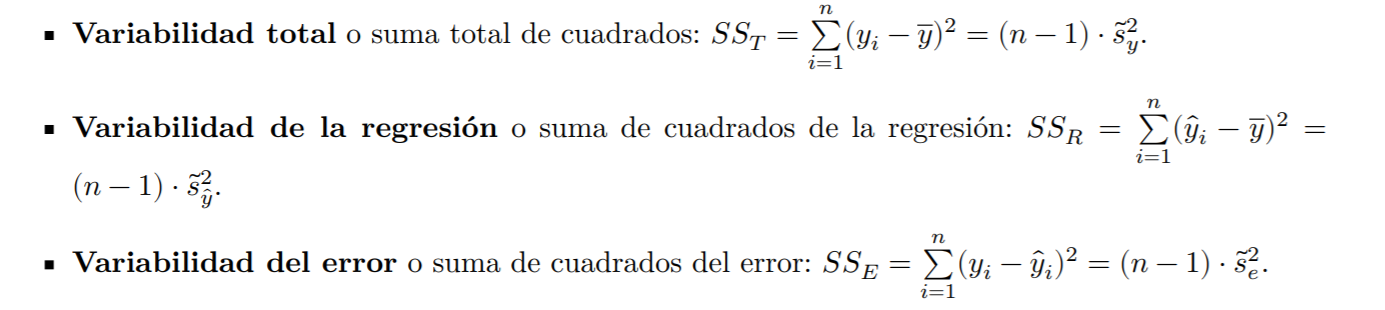
\includegraphics[width=400px]{formulas_regre}

\begin{Shaded}
\begin{Highlighting}[]
\NormalTok{SST=}\KeywordTok{sum}\NormalTok{((y}\OperatorTok{-}\KeywordTok{mean}\NormalTok{(y))}\OperatorTok{^}\DecValTok{2}\NormalTok{)}
\NormalTok{SST}
\end{Highlighting}
\end{Shaded}

\begin{verbatim}
## [1] 131.5
\end{verbatim}

\begin{Shaded}
\begin{Highlighting}[]
\KeywordTok{mean}\NormalTok{(y_est)}
\end{Highlighting}
\end{Shaded}

\begin{verbatim}
## [1] -0.5
\end{verbatim}

\begin{Shaded}
\begin{Highlighting}[]
\KeywordTok{mean}\NormalTok{(y)}\CommentTok{#media estimados regresion igual a media variable y}
\end{Highlighting}
\end{Shaded}

\begin{verbatim}
## [1] -0.5
\end{verbatim}

\begin{Shaded}
\begin{Highlighting}[]
\NormalTok{SSR=}\KeywordTok{sum}\NormalTok{((y_est}\OperatorTok{-}\KeywordTok{mean}\NormalTok{(y))}\OperatorTok{^}\DecValTok{2}\NormalTok{)}
\NormalTok{SSR}
\end{Highlighting}
\end{Shaded}

\begin{verbatim}
## [1] 126.075
\end{verbatim}

\begin{Shaded}
\begin{Highlighting}[]
\NormalTok{SSE}\CommentTok{# ya lo había a calculado}
\end{Highlighting}
\end{Shaded}

\begin{verbatim}
## [1] 5.425
\end{verbatim}

\begin{Shaded}
\begin{Highlighting}[]
\NormalTok{SST}\OperatorTok{-}\NormalTok{SSR}\CommentTok{# da lo mismo pues SST=SSR+SSE }
\end{Highlighting}
\end{Shaded}

\begin{verbatim}
## [1] 5.425
\end{verbatim}

\begin{Shaded}
\begin{Highlighting}[]
\NormalTok{R2=SSR}\OperatorTok{/}\NormalTok{SST}
\NormalTok{R2}
\end{Highlighting}
\end{Shaded}

\begin{verbatim}
## [1] 0.9587452
\end{verbatim}

\begin{Shaded}
\begin{Highlighting}[]
\KeywordTok{cor}\NormalTok{(x,y)}
\end{Highlighting}
\end{Shaded}

\begin{verbatim}
## [1] 0.9791554
\end{verbatim}

\begin{Shaded}
\begin{Highlighting}[]
\KeywordTok{cor}\NormalTok{(x,y)}\OperatorTok{^}\DecValTok{2}\CommentTok{# en el caso regre simp`le R2=cor(xy)^2}
\end{Highlighting}
\end{Shaded}

\begin{verbatim}
## [1] 0.9587452
\end{verbatim}

\hypertarget{problema-5-distribuciuxf3n-de-los-grados-de-un-grafo-de-contactos.}{%
\subsection{Problema 5: Distribución de los grados de un grafo de
contactos.}\label{problema-5-distribuciuxf3n-de-los-grados-de-un-grafo-de-contactos.}}

En el artículo de A. Broder et al.,
\href{http://snap.stanford.edu/class/cs224w-readings/broder00bowtie.pdf}{Graph
structure in the Web. Computer Networks 33, 309 (2000)}.

Se recopiló el número de enlaces a sitios web encontrados en un rastreo
web de 1997 de aproximadamente 200 millones de páginas web,

Con el se construyó una
\href{http://tuvalu.santafe.edu/~aaronc/powerlaws/data/weblinks.hist}{tabla}
con la frecuencia de sitios por número de enlaces. El código siguiente
carga del enlace que han puesto los autores del artículo

\begin{Shaded}
\begin{Highlighting}[]
\NormalTok{data_links=}\KeywordTok{read.table}\NormalTok{(}\StringTok{"http://tuvalu.santafe.edu/~aaronc/powerlaws/data/weblinks.hist"}\NormalTok{,}\DataTypeTok{header=}\OtherTok{TRUE}\NormalTok{)}
\KeywordTok{head}\NormalTok{(data_links)}
\end{Highlighting}
\end{Shaded}

\begin{verbatim}
##   degree frequency
## 1      0  35159835
## 2      1 106649769
## 3      2  40711748
## 4      3  22648832
## 5      4  12617832
## 6      5   8188854
\end{verbatim}

\begin{Shaded}
\begin{Highlighting}[]
\KeywordTok{str}\NormalTok{(data_links)}
\end{Highlighting}
\end{Shaded}

\begin{verbatim}
## 'data.frame':    14480 obs. of  2 variables:
##  $ degree   : int  0 1 2 3 4 5 6 7 8 9 ...
##  $ frequency: int  35159835 106649769 40711748 22648832 12617832 8188854 6438634 4690068 4954649 3731928 ...
\end{verbatim}

\begin{Shaded}
\begin{Highlighting}[]
\CommentTok{# eliminamos la páginas con menos de 8 enlaces  enlaces y las de más de 1000 enlaces}
\NormalTok{data_links_central=data_links[data_links}\OperatorTok{$}\NormalTok{degree}\OperatorTok{>}\DecValTok{8}\OperatorTok{&}\NormalTok{data_links}\OperatorTok{$}\NormalTok{degree}\OperatorTok{<}\DecValTok{10}\OperatorTok{^}\DecValTok{3}\NormalTok{,]}
\KeywordTok{head}\NormalTok{(data_links_central)}
\end{Highlighting}
\end{Shaded}

\begin{verbatim}
##    degree frequency
## 10      9   3731928
## 11     10   3036333
## 12     11   2496648
## 13     12   2119312
## 14     13   1790068
## 15     14   1546579
\end{verbatim}

\begin{Shaded}
\begin{Highlighting}[]
\KeywordTok{tail}\NormalTok{(data_links_central)}
\end{Highlighting}
\end{Shaded}

\begin{verbatim}
##      degree frequency
## 995     994       213
## 996     995       193
## 997     996       157
## 998     997       137
## 999     998       178
## 1000    999       153
\end{verbatim}

El siguiente código calcula las regresiones exponecial, potencial y
lineal (en algún orden) de las frecuencias (\texttt{frequency}) contra
los enlaces (\texttt{degree}).

\begin{Shaded}
\begin{Highlighting}[]
\NormalTok{sol1=}\KeywordTok{lm}\NormalTok{(frequency}\OperatorTok{~}\StringTok{ }\NormalTok{degree,}\DataTypeTok{data=}\NormalTok{data_links_central)}
\KeywordTok{summary}\NormalTok{(sol1)}
\end{Highlighting}
\end{Shaded}

\begin{verbatim}
## 
## Call:
## lm(formula = frequency ~ degree, data = data_links_central)
## 
## Residuals:
##     Min      1Q  Median      3Q     Max 
##  -96861  -69548  -25033   22374 3598744 
## 
## Coefficients:
##              Estimate Std. Error t value            Pr(>|t|)    
## (Intercept) 134974.49   13778.17   9.796 <0.0000000000000002 ***
## degree        -198.98      23.77  -8.369 <0.0000000000000002 ***
## ---
## Signif. codes:  0 '***' 0.001 '**' 0.01 '*' 0.05 '.' 0.1 ' ' 1
## 
## Residual standard error: 214100 on 989 degrees of freedom
## Multiple R-squared:  0.06614,    Adjusted R-squared:  0.06519 
## F-statistic: 70.04 on 1 and 989 DF,  p-value: < 0.00000000000000022
\end{verbatim}

\begin{Shaded}
\begin{Highlighting}[]
\NormalTok{sol2=}\KeywordTok{lm}\NormalTok{(}\KeywordTok{log10}\NormalTok{(frequency)}\OperatorTok{~}\StringTok{ }\NormalTok{degree,}\DataTypeTok{data=}\NormalTok{data_links_central)}
\KeywordTok{summary}\NormalTok{(sol2)}
\end{Highlighting}
\end{Shaded}

\begin{verbatim}
## 
## Call:
## lm(formula = log10(frequency) ~ degree, data = data_links_central)
## 
## Residuals:
##      Min       1Q   Median       3Q      Max 
## -0.43758 -0.26558 -0.07671  0.16681  2.13097 
## 
## Coefficients:
##                Estimate  Std. Error t value            Pr(>|t|)    
## (Intercept)  4.46504979  0.02381018  187.53 <0.0000000000000002 ***
## degree      -0.00267658  0.00004109  -65.15 <0.0000000000000002 ***
## ---
## Signif. codes:  0 '***' 0.001 '**' 0.01 '*' 0.05 '.' 0.1 ' ' 1
## 
## Residual standard error: 0.37 on 989 degrees of freedom
## Multiple R-squared:  0.811,  Adjusted R-squared:  0.8108 
## F-statistic:  4244 on 1 and 989 DF,  p-value: < 0.00000000000000022
\end{verbatim}

\begin{Shaded}
\begin{Highlighting}[]
\NormalTok{sol3=}\KeywordTok{lm}\NormalTok{(}\KeywordTok{log10}\NormalTok{(frequency)}\OperatorTok{~}\StringTok{ }\KeywordTok{log10}\NormalTok{(degree),}\DataTypeTok{data=}\NormalTok{data_links_central)}
\KeywordTok{summary}\NormalTok{(sol3)}
\end{Highlighting}
\end{Shaded}

\begin{verbatim}
## 
## Call:
## lm(formula = log10(frequency) ~ log10(degree), data = data_links_central)
## 
## Residuals:
##      Min       1Q   Median       3Q      Max 
## -0.21376 -0.04747 -0.01555  0.01958  0.73976 
## 
## Coefficients:
##                Estimate Std. Error t value            Pr(>|t|)    
## (Intercept)    8.722036   0.020623   422.9 <0.0000000000000002 ***
## log10(degree) -2.170129   0.007894  -274.9 <0.0000000000000002 ***
## ---
## Signif. codes:  0 '***' 0.001 '**' 0.01 '*' 0.05 '.' 0.1 ' ' 1
## 
## Residual standard error: 0.09674 on 989 degrees of freedom
## Multiple R-squared:  0.9871, Adjusted R-squared:  0.9871 
## F-statistic: 7.557e+04 on 1 and 989 DF,  p-value: < 0.00000000000000022
\end{verbatim}

Ahora dibujamos los gráficos adecuados a cada modelo

\begin{Shaded}
\begin{Highlighting}[]
\KeywordTok{plot}\NormalTok{(data_links_central,}\DataTypeTok{main=}\StringTok{"Modelo .........."}\NormalTok{)}
\KeywordTok{abline}\NormalTok{(sol1,}\DataTypeTok{col=}\StringTok{"red"}\NormalTok{)}
\end{Highlighting}
\end{Shaded}

\includegraphics{Entrega4_ENUNCIADO_SOLUCIONES_files/figure-latex/unnamed-chunk-26-1.pdf}

\begin{Shaded}
\begin{Highlighting}[]
\KeywordTok{plot}\NormalTok{(data_links_central,}\DataTypeTok{main=}\StringTok{"Modelo .........."}\NormalTok{,}\DataTypeTok{log=}\StringTok{"y"}\NormalTok{)}
\KeywordTok{abline}\NormalTok{(sol2,}\DataTypeTok{col=}\StringTok{"red"}\NormalTok{)}
\end{Highlighting}
\end{Shaded}

\includegraphics{Entrega4_ENUNCIADO_SOLUCIONES_files/figure-latex/unnamed-chunk-26-2.pdf}

\begin{Shaded}
\begin{Highlighting}[]
\KeywordTok{plot}\NormalTok{(data_links_central,}\DataTypeTok{main=}\StringTok{"Modelo .........."}\NormalTok{,}\DataTypeTok{log=}\StringTok{"xy"}\NormalTok{)}
\KeywordTok{abline}\NormalTok{(sol3,}\DataTypeTok{col=}\StringTok{"red"}\NormalTok{)}
\end{Highlighting}
\end{Shaded}

\includegraphics{Entrega4_ENUNCIADO_SOLUCIONES_files/figure-latex/unnamed-chunk-26-3.pdf}

Se pide:

\begin{enumerate}
\def\labelenumi{\arabic{enumi}.}
\tightlist
\item
  Explicad el modelo de regresión que calcula cada función \texttt{lm}
\item
  ¿Qué modelo y en función de qué parámetros es el mejor?
\item
  Para el mejor modelo calcular los coeficientes en las unidades
  originales y escribir la ecuación del modelos.
\end{enumerate}

\hypertarget{soluciuxf3n-4}{%
\subsubsection{Solución}\label{soluciuxf3n-4}}

\textbf{Apartado 1}

Los modelos son

\begin{Shaded}
\begin{Highlighting}[]
\NormalTok{sol1=}\KeywordTok{lm}\NormalTok{(frequency}\OperatorTok{~}\StringTok{ }\NormalTok{degree,}\DataTypeTok{data=}\NormalTok{data_links_central)}
\KeywordTok{summary}\NormalTok{(sol1)}
\end{Highlighting}
\end{Shaded}

\begin{verbatim}
## 
## Call:
## lm(formula = frequency ~ degree, data = data_links_central)
## 
## Residuals:
##     Min      1Q  Median      3Q     Max 
##  -96861  -69548  -25033   22374 3598744 
## 
## Coefficients:
##              Estimate Std. Error t value            Pr(>|t|)    
## (Intercept) 134974.49   13778.17   9.796 <0.0000000000000002 ***
## degree        -198.98      23.77  -8.369 <0.0000000000000002 ***
## ---
## Signif. codes:  0 '***' 0.001 '**' 0.01 '*' 0.05 '.' 0.1 ' ' 1
## 
## Residual standard error: 214100 on 989 degrees of freedom
## Multiple R-squared:  0.06614,    Adjusted R-squared:  0.06519 
## F-statistic: 70.04 on 1 and 989 DF,  p-value: < 0.00000000000000022
\end{verbatim}

\begin{Shaded}
\begin{Highlighting}[]
\NormalTok{sol2=}\KeywordTok{lm}\NormalTok{(}\KeywordTok{log10}\NormalTok{(frequency)}\OperatorTok{~}\StringTok{ }\NormalTok{degree,}\DataTypeTok{data=}\NormalTok{data_links_central)}
\KeywordTok{summary}\NormalTok{(sol2)}
\end{Highlighting}
\end{Shaded}

\begin{verbatim}
## 
## Call:
## lm(formula = log10(frequency) ~ degree, data = data_links_central)
## 
## Residuals:
##      Min       1Q   Median       3Q      Max 
## -0.43758 -0.26558 -0.07671  0.16681  2.13097 
## 
## Coefficients:
##                Estimate  Std. Error t value            Pr(>|t|)    
## (Intercept)  4.46504979  0.02381018  187.53 <0.0000000000000002 ***
## degree      -0.00267658  0.00004109  -65.15 <0.0000000000000002 ***
## ---
## Signif. codes:  0 '***' 0.001 '**' 0.01 '*' 0.05 '.' 0.1 ' ' 1
## 
## Residual standard error: 0.37 on 989 degrees of freedom
## Multiple R-squared:  0.811,  Adjusted R-squared:  0.8108 
## F-statistic:  4244 on 1 and 989 DF,  p-value: < 0.00000000000000022
\end{verbatim}

\begin{Shaded}
\begin{Highlighting}[]
\NormalTok{sol3=}\KeywordTok{lm}\NormalTok{(}\KeywordTok{log10}\NormalTok{(frequency)}\OperatorTok{~}\StringTok{ }\KeywordTok{log10}\NormalTok{(degree),}\DataTypeTok{data=}\NormalTok{data_links_central)}
\KeywordTok{summary}\NormalTok{(sol3)}
\end{Highlighting}
\end{Shaded}

\begin{verbatim}
## 
## Call:
## lm(formula = log10(frequency) ~ log10(degree), data = data_links_central)
## 
## Residuals:
##      Min       1Q   Median       3Q      Max 
## -0.21376 -0.04747 -0.01555  0.01958  0.73976 
## 
## Coefficients:
##                Estimate Std. Error t value            Pr(>|t|)    
## (Intercept)    8.722036   0.020623   422.9 <0.0000000000000002 ***
## log10(degree) -2.170129   0.007894  -274.9 <0.0000000000000002 ***
## ---
## Signif. codes:  0 '***' 0.001 '**' 0.01 '*' 0.05 '.' 0.1 ' ' 1
## 
## Residual standard error: 0.09674 on 989 degrees of freedom
## Multiple R-squared:  0.9871, Adjusted R-squared:  0.9871 
## F-statistic: 7.557e+04 on 1 and 989 DF,  p-value: < 0.00000000000000022
\end{verbatim}

Así que

\begin{itemize}
\tightlist
\item
  el primero es \(frequency = b_0+b_1\cdot degree\) que el el modelo
  LINEAL que resuelve la fución \texttt{lm}.
\item
  el segundo es \(\log_{10}(frequency) = b_0+b_1\cdot degree\) que
  operando adecuadamente es
  \(10^\log_{10}(frequency)=10^{b_0}\cdot 10^{b_1\cdot degree}\)
  operando obtenemos que el modelo final es un modelo EXPONENCIAL
  \(frequency=10^{b_0}\cdot \left(10^{b_1}\right)^{degree}\).
\item
  el tercer modelo es
  \(\log_{10}(frequency) = b_0+b_1\cdot \log_{10}(degree)\) que
  despejando es
  \(10^\log_{10}(frequency)=10^{b_0}\cdot \left(10^\left(\log_{10}(degree)\righ)\right)^{b_1}\)
  operando obtenemos que el modelo final es un modelo POTENCIAL
  \(frequency=10^{b_0}\cdot degree^{b_1}.\)
\end{itemize}

Los dibujos con el título adecuado son

\begin{Shaded}
\begin{Highlighting}[]
\KeywordTok{plot}\NormalTok{(data_links_central,}\DataTypeTok{main=}\StringTok{"Modelo lineal"}\NormalTok{)}
\KeywordTok{abline}\NormalTok{(sol1,}\DataTypeTok{col=}\StringTok{"red"}\NormalTok{)}
\end{Highlighting}
\end{Shaded}

\includegraphics{Entrega4_ENUNCIADO_SOLUCIONES_files/figure-latex/unnamed-chunk-28-1.pdf}

\begin{Shaded}
\begin{Highlighting}[]
\KeywordTok{plot}\NormalTok{(data_links_central,}\DataTypeTok{main=}\StringTok{"Modelo exponencial"}\NormalTok{,}\DataTypeTok{log=}\StringTok{"y"}\NormalTok{)}
\KeywordTok{abline}\NormalTok{(sol2,}\DataTypeTok{col=}\StringTok{"red"}\NormalTok{)}
\end{Highlighting}
\end{Shaded}

\includegraphics{Entrega4_ENUNCIADO_SOLUCIONES_files/figure-latex/unnamed-chunk-28-2.pdf}

\begin{Shaded}
\begin{Highlighting}[]
\KeywordTok{plot}\NormalTok{(data_links_central,}\DataTypeTok{main=}\StringTok{"Modelo potencial"}\NormalTok{,}\DataTypeTok{log=}\StringTok{"xy"}\NormalTok{)}
\KeywordTok{abline}\NormalTok{(sol3,}\DataTypeTok{col=}\StringTok{"red"}\NormalTok{)}
\end{Highlighting}
\end{Shaded}

\includegraphics{Entrega4_ENUNCIADO_SOLUCIONES_files/figure-latex/unnamed-chunk-28-3.pdf}

Con lo que hemos visto el modelo con mejor \(R^2\) es el mejor

\begin{Shaded}
\begin{Highlighting}[]
\KeywordTok{summary}\NormalTok{(sol1)}\OperatorTok{$}\NormalTok{r.squared}
\end{Highlighting}
\end{Shaded}

\begin{verbatim}
## [1] 0.06613879
\end{verbatim}

\begin{Shaded}
\begin{Highlighting}[]
\KeywordTok{summary}\NormalTok{(sol2)}\OperatorTok{$}\NormalTok{r.squared}
\end{Highlighting}
\end{Shaded}

\begin{verbatim}
## [1] 0.8110118
\end{verbatim}

\begin{Shaded}
\begin{Highlighting}[]
\KeywordTok{summary}\NormalTok{(sol3)}\OperatorTok{$}\NormalTok{r.squared}
\end{Highlighting}
\end{Shaded}

\begin{verbatim}
## [1] 0.9870815
\end{verbatim}

Así que el mejor modelo es el tercero el pontecial pues su \(R^2\) es
muy alto

\textbf{Apartado 3}

Calcularemos la ecuación del modelo para las unidades originales sin
transformaciones logarítmicas.

Recordemos el resultado de la \texttt{sol3}

\begin{Shaded}
\begin{Highlighting}[]
\KeywordTok{summary}\NormalTok{(sol3)}
\end{Highlighting}
\end{Shaded}

\begin{verbatim}
## 
## Call:
## lm(formula = log10(frequency) ~ log10(degree), data = data_links_central)
## 
## Residuals:
##      Min       1Q   Median       3Q      Max 
## -0.21376 -0.04747 -0.01555  0.01958  0.73976 
## 
## Coefficients:
##                Estimate Std. Error t value            Pr(>|t|)    
## (Intercept)    8.722036   0.020623   422.9 <0.0000000000000002 ***
## log10(degree) -2.170129   0.007894  -274.9 <0.0000000000000002 ***
## ---
## Signif. codes:  0 '***' 0.001 '**' 0.01 '*' 0.05 '.' 0.1 ' ' 1
## 
## Residual standard error: 0.09674 on 989 degrees of freedom
## Multiple R-squared:  0.9871, Adjusted R-squared:  0.9871 
## F-statistic: 7.557e+04 on 1 and 989 DF,  p-value: < 0.00000000000000022
\end{verbatim}

Los estimadores son \(b_0=8.722036\) y \(b_1=-2.170129\) el modelo es
\(frequency=10^{b_0}\cdot degree^{b_1}\). Sustitutendo los valores el
modelo obtenemos \(frequency=10^{8.722036}\cdot degree^{-2.170129}\),
finalmente operando

\[frequency=527273566.93254\cdot degree^{-2.170129}.\]

No se pedía en el ejercicio pero hacemos el dibujo de los datos y la
ecuación en las unidades originales

\begin{Shaded}
\begin{Highlighting}[]
\NormalTok{frequency=data_links_central}\OperatorTok{$}\NormalTok{frequency}
\NormalTok{degree=data_links_central}\OperatorTok{$}\NormalTok{degree}
\NormalTok{potencial=}\ControlFlowTok{function}\NormalTok{(x) }\DecValTok{10}\OperatorTok{^}\NormalTok{(}\FloatTok{8.722036}\NormalTok{)}\OperatorTok{*}\NormalTok{x}\OperatorTok{^}\NormalTok{(}\OperatorTok{-}\FloatTok{2.170129}\NormalTok{)}
\KeywordTok{plot}\NormalTok{(degree,frequency,}\DataTypeTok{main=}\StringTok{"Modelo potencial"}\NormalTok{,}\DataTypeTok{xlab=}\StringTok{"degree"}\NormalTok{,}\DataTypeTok{ylab=}\StringTok{"frequency"}\NormalTok{)}
\KeywordTok{curve}\NormalTok{(potencial,}\DataTypeTok{xlim=}\KeywordTok{c}\NormalTok{(}\DecValTok{0}\NormalTok{,}\DecValTok{1000}\NormalTok{),}\DataTypeTok{ylim=}\KeywordTok{c}\NormalTok{(}\DecValTok{0}\NormalTok{,}\DecValTok{3731928}\NormalTok{),}\DataTypeTok{col=}\StringTok{"red"}\NormalTok{,}\DataTypeTok{add=}\OtherTok{TRUE}\NormalTok{)}
\end{Highlighting}
\end{Shaded}

\includegraphics{Entrega4_ENUNCIADO_SOLUCIONES_files/figure-latex/unnamed-chunk-31-1.pdf}

\end{document}
